\chapter{Verbs}

Verbs listed here come from CPED. Fortunately, the dictionary has already provided us the composition of verbs and their related forms. New students can learn a lot just by going through these lists.

We have only two main options: to see the main (canonical) verb form (singular, present, third-person, active), typically those ending with \pali{-ti}, and the rest. In main verbs, you can also filter the list by the verbs themselves, their root and prefix, their ending component (\pali{paccaya})\footnote{The name of roots and \pali{paccaya}s can be slightly different from Kaccāyana/Saddanīti's convention.}, or their meaning. The use is straightforward. Figure \ref{fig:verbs-main} shows a search result.

\begin{figure}[!hbt]
\centering
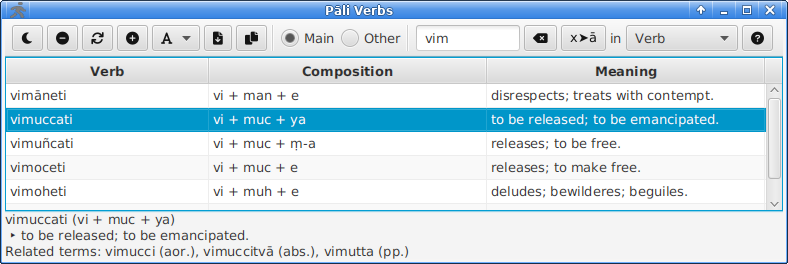
\includegraphics[width=0.9\linewidth]{images/verbs-main.png}\\
\caption{Results of main verbs}
\label{fig:verbs-main}
\end{figure}

In other verb forms, you have to choose the group you want (see Figure \ref{fig:verbs-other}). The names of verb forms here come directly from the dictionary. So, some name may look unfamiliar, for example, \emph{Potential Participle} is called commonly by other textbooks as \emph{Future Passive Participle}. 

\begin{figure}[!hbt]
\centering
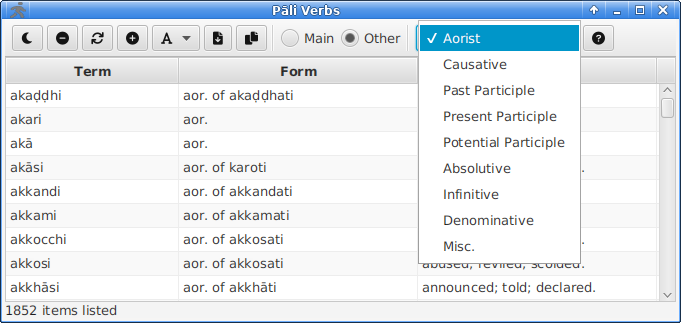
\includegraphics[width=0.9\linewidth]{images/verbs-other.png}\\
\caption{Options of other verb forms}
\label{fig:verbs-other}
\end{figure}

If you cannot find some verbs, or some forms look dubious to you, please check them against DPD (see Chapter \ref{chap:dpd}) or MDPD in Dict window, which has a more exhaustive list.

